\documentclass[a4paper,  11pt]{ctexart}
\usepackage{srcltx,graphicx}
\usepackage{amsmath, amssymb, amsthm}
\usepackage{color}
\usepackage{lscape}
\usepackage{multirow}
\usepackage{psfrag}
\usepackage{diagbox}
\usepackage[hang]{subfigure}
\usepackage{float}
\usepackage[colorlinks,linkcolor=black,anchorcolor=blue,citecolor=green]{hyperref}

\newtheorem{theorem}{Theorem}
\newtheorem{lemma}{Lemma}
\newtheorem{definition}{Definition}
\newtheorem{comment}{Comment}
\newtheorem{conjecture}{Conjecture}

\newcommand\bbR{\mathbb{R}}
\newcommand\bbN{\mathbb{N}}
\newcommand\bbC{\mathbb{C}}
\newcommand\bx{\boldsymbol{x}}
\newcommand\dd{\,\mathrm{d}}

\newcommand\diag{\mathrm{diag}}
\newcommand\tr{\mthrm{tr}}

\setlength{\oddsidemargin}{0cm}
\setlength{\evensidemargin}{0cm}
\setlength{\textwidth}{150mm}
\setlength{\textheight}{230mm}

\newcommand\note[2]{{{\bf #1}\color{red} [ {\it #2} ]}}
%\newcommand\note[2]{{ #1 }} % using this line in the formal version

\newcommand\pd[2]{\dfrac{\partial {#1}}{\partial {#2}}}
\newcommand\od[2]{\dfrac{\dd {#1}}{\dd {#2}}}
\newcommand{\bm}[1]{\mbox{\boldmath{$#1$}}}

\begin{document}
\title{有限体积格式不同数值通量和限制器的比较}
\author{郑灵超}  
\maketitle
% \tableofcontents
% \newpage

\section{理论分析}
\subsection{有限体积格式} 
对于守恒率方程 
\begin{equation}
  \label{eq:ConservationLaws}
  \pd{U}{t}+\nabla \cdot F(U) = 0
\end{equation}  
将其在空间区域$\Omega$积分,得
\[  
\pd{(\int_{\Omega}U\dd\bx)}{t} + \int_{\Omega} \nabla \cdot F(U)\dd\bx = 0
\]
令 $\bar{U}$为$U$在区域$\Omega$上的积分平均,则
\[  
    |\Omega|\pd{\bar{U}}{t} + \int_{\partial\Omega} F(U)\cdot \bm{n}
    \dd S = 0
\]

我们假设$\Omega_i$表示一个多面体网格,其相邻网格为$\Omega_{i,j}$,
$\Omega_i$与$\Omega_{i,j}$的交界面为$S_j$.
\[  
   |\Omega_i|\pd{\bar{U}}{t} + \sum_{j} \int_{S_j} F(U)\cdot \bm{n}
   \dd S = 0
\]
\[   
|\Omega_i|\pd{\bar{U}}{t} + \sum_{j} \hat{F}(\Omega_i,\Omega_{i,i_j})= 0 
\] 
\subsection{数值通量}
\subsection{重构}


\section{数值实验}
\subsection{一维问题}
\subsubsection{线性对流方程}
我们先选取一个简单的线性对流方程
\[ 
    u_t + u_x = 0
\] 
计算区域为$[-1,1]$,采用周期边界条件。初始值为 
\begin{figure}[H]
  \begin{center}
    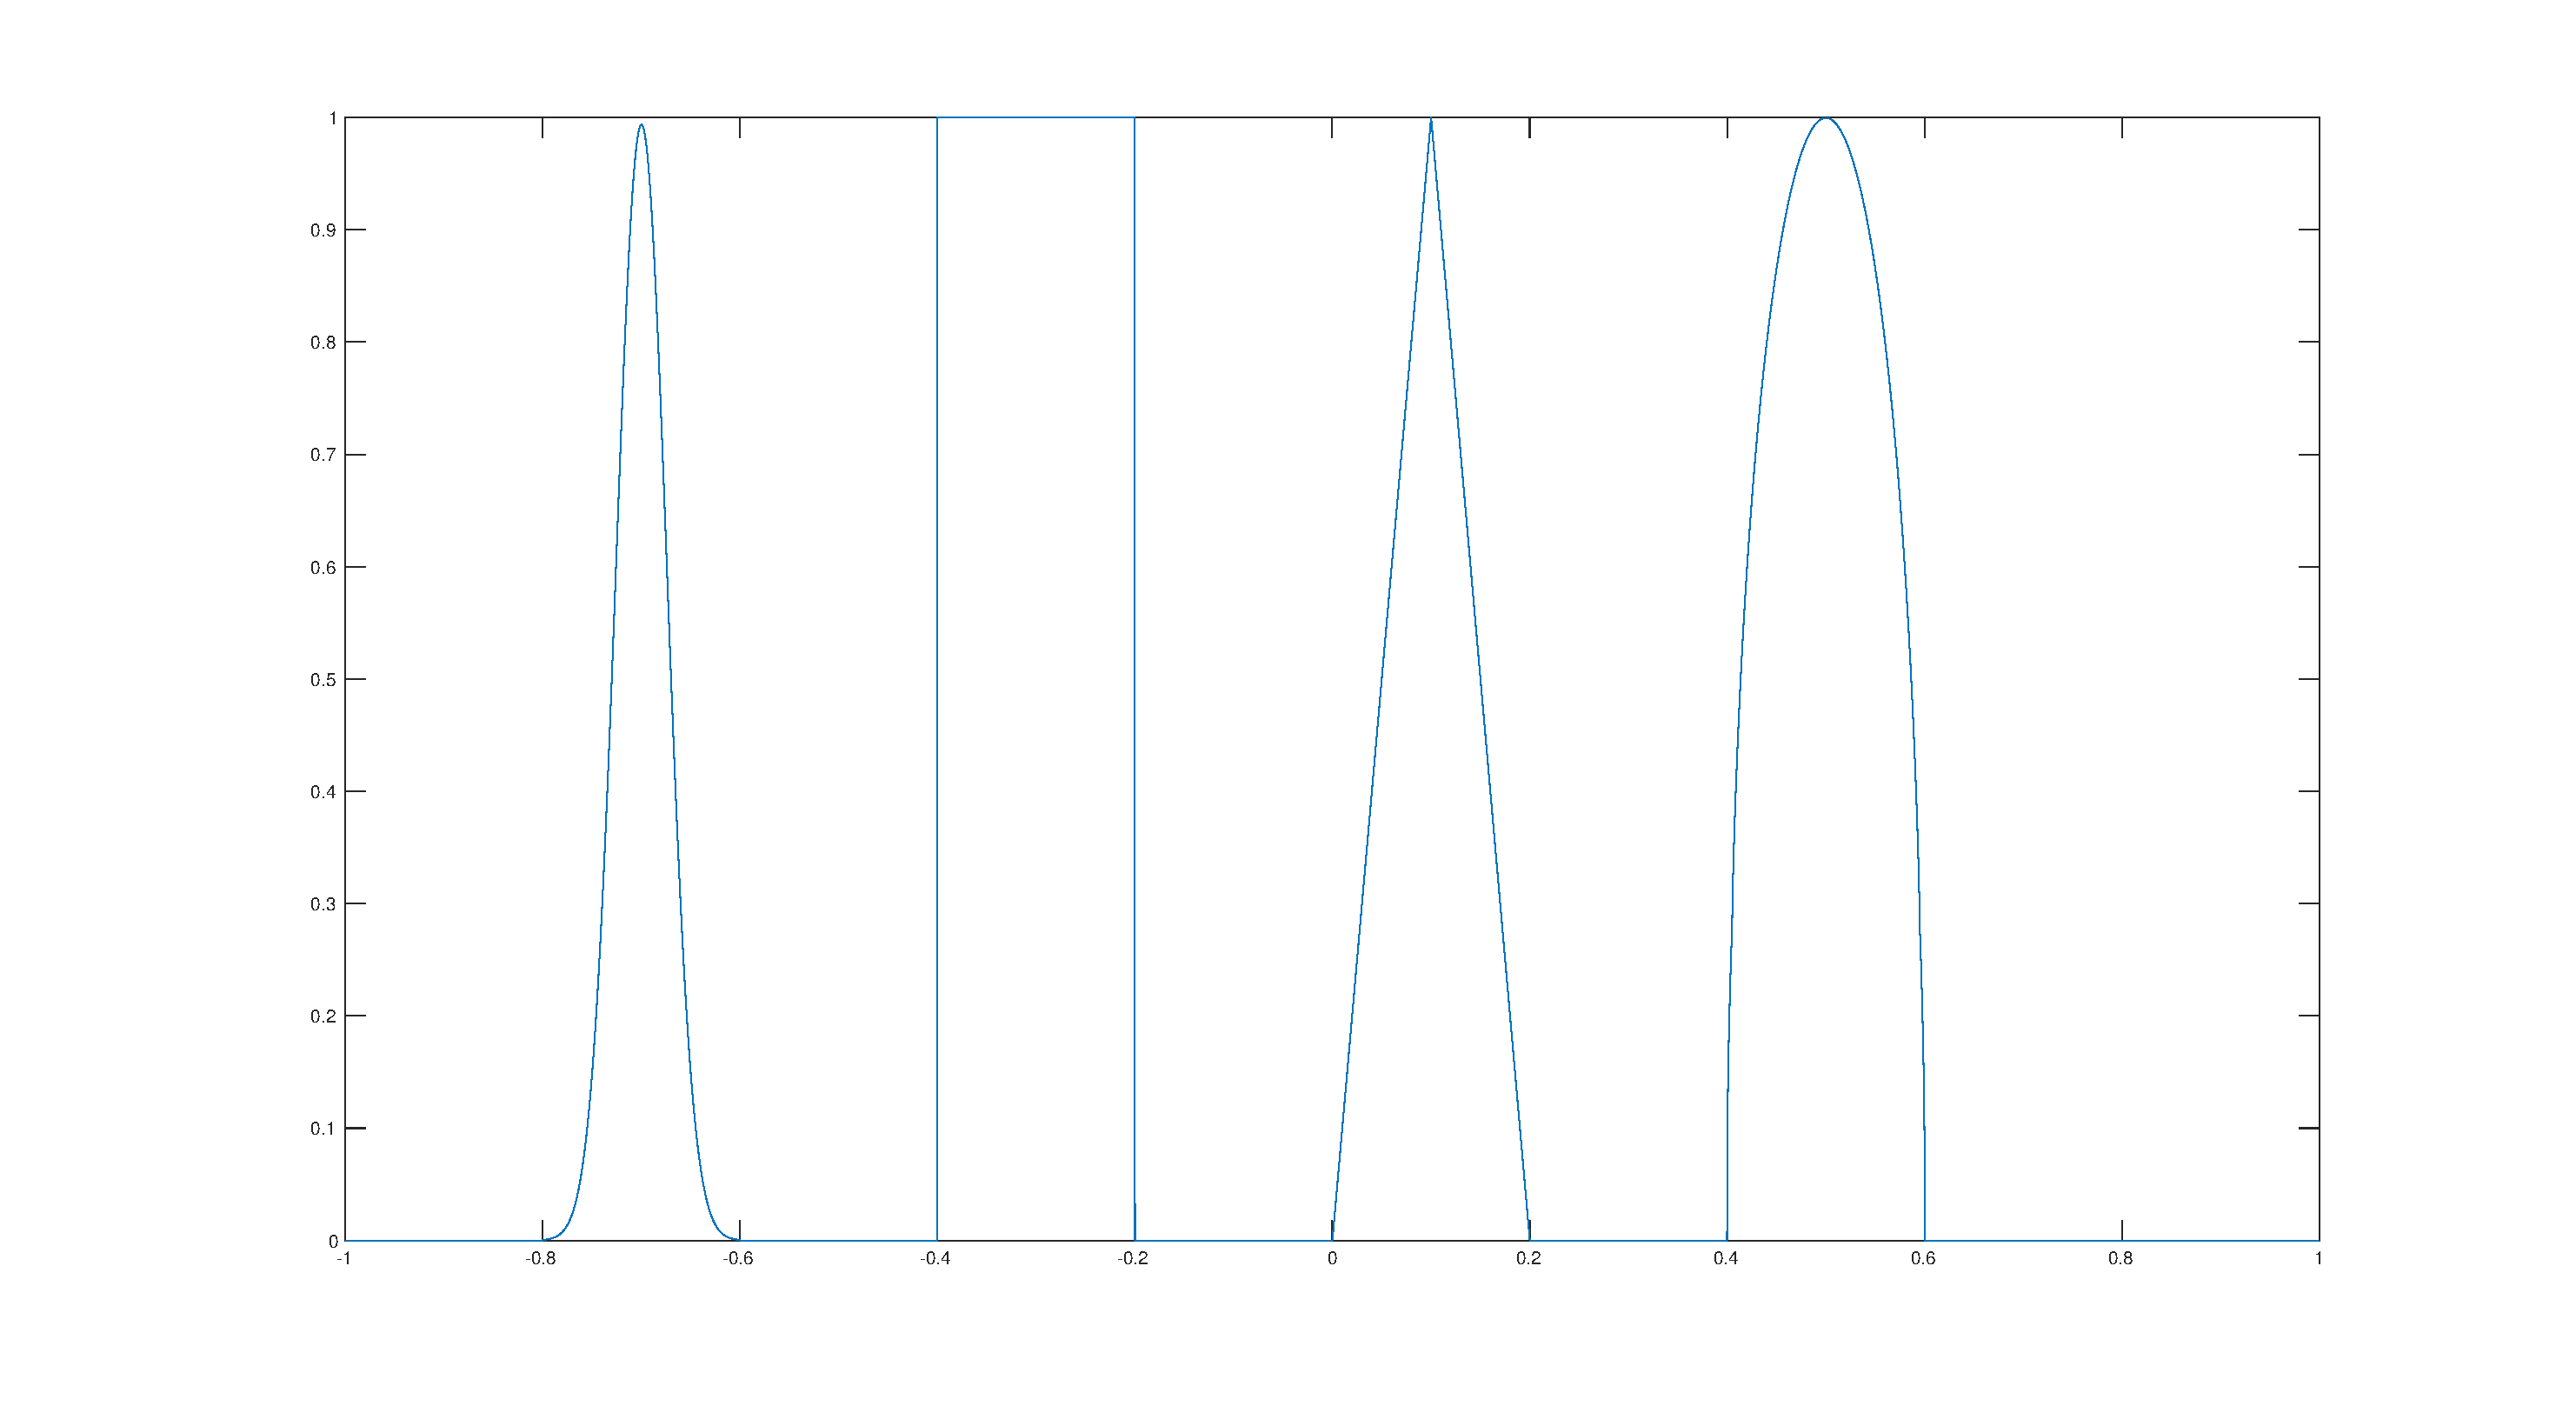
\includegraphics[width=\textwidth]{./images/advection_t0.eps}
  \end{center}
  \caption{初始值}
\end{figure}
终止时刻$t=8$,可以预期真解与初始值是一致的。以下为不同通量的计算结果:
\begin{figure}[H]
  \subfigure[LF]{
    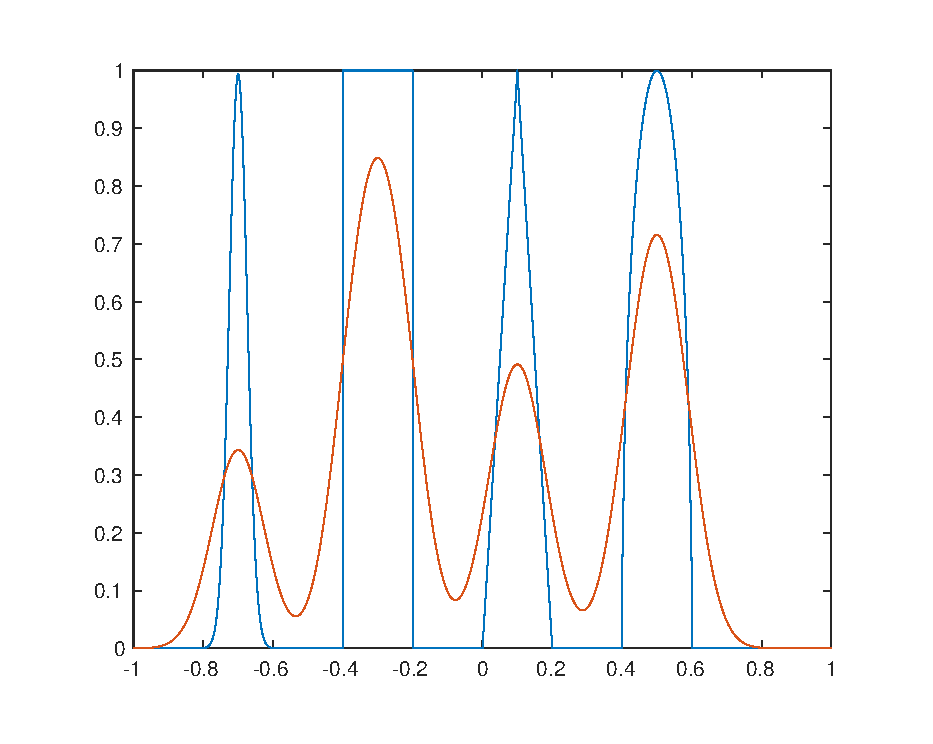
\includegraphics[width=0.45\textwidth, height=0.225\textheight]{./images/advection_LF.eps}
  }
  \subfigure[LW]{
    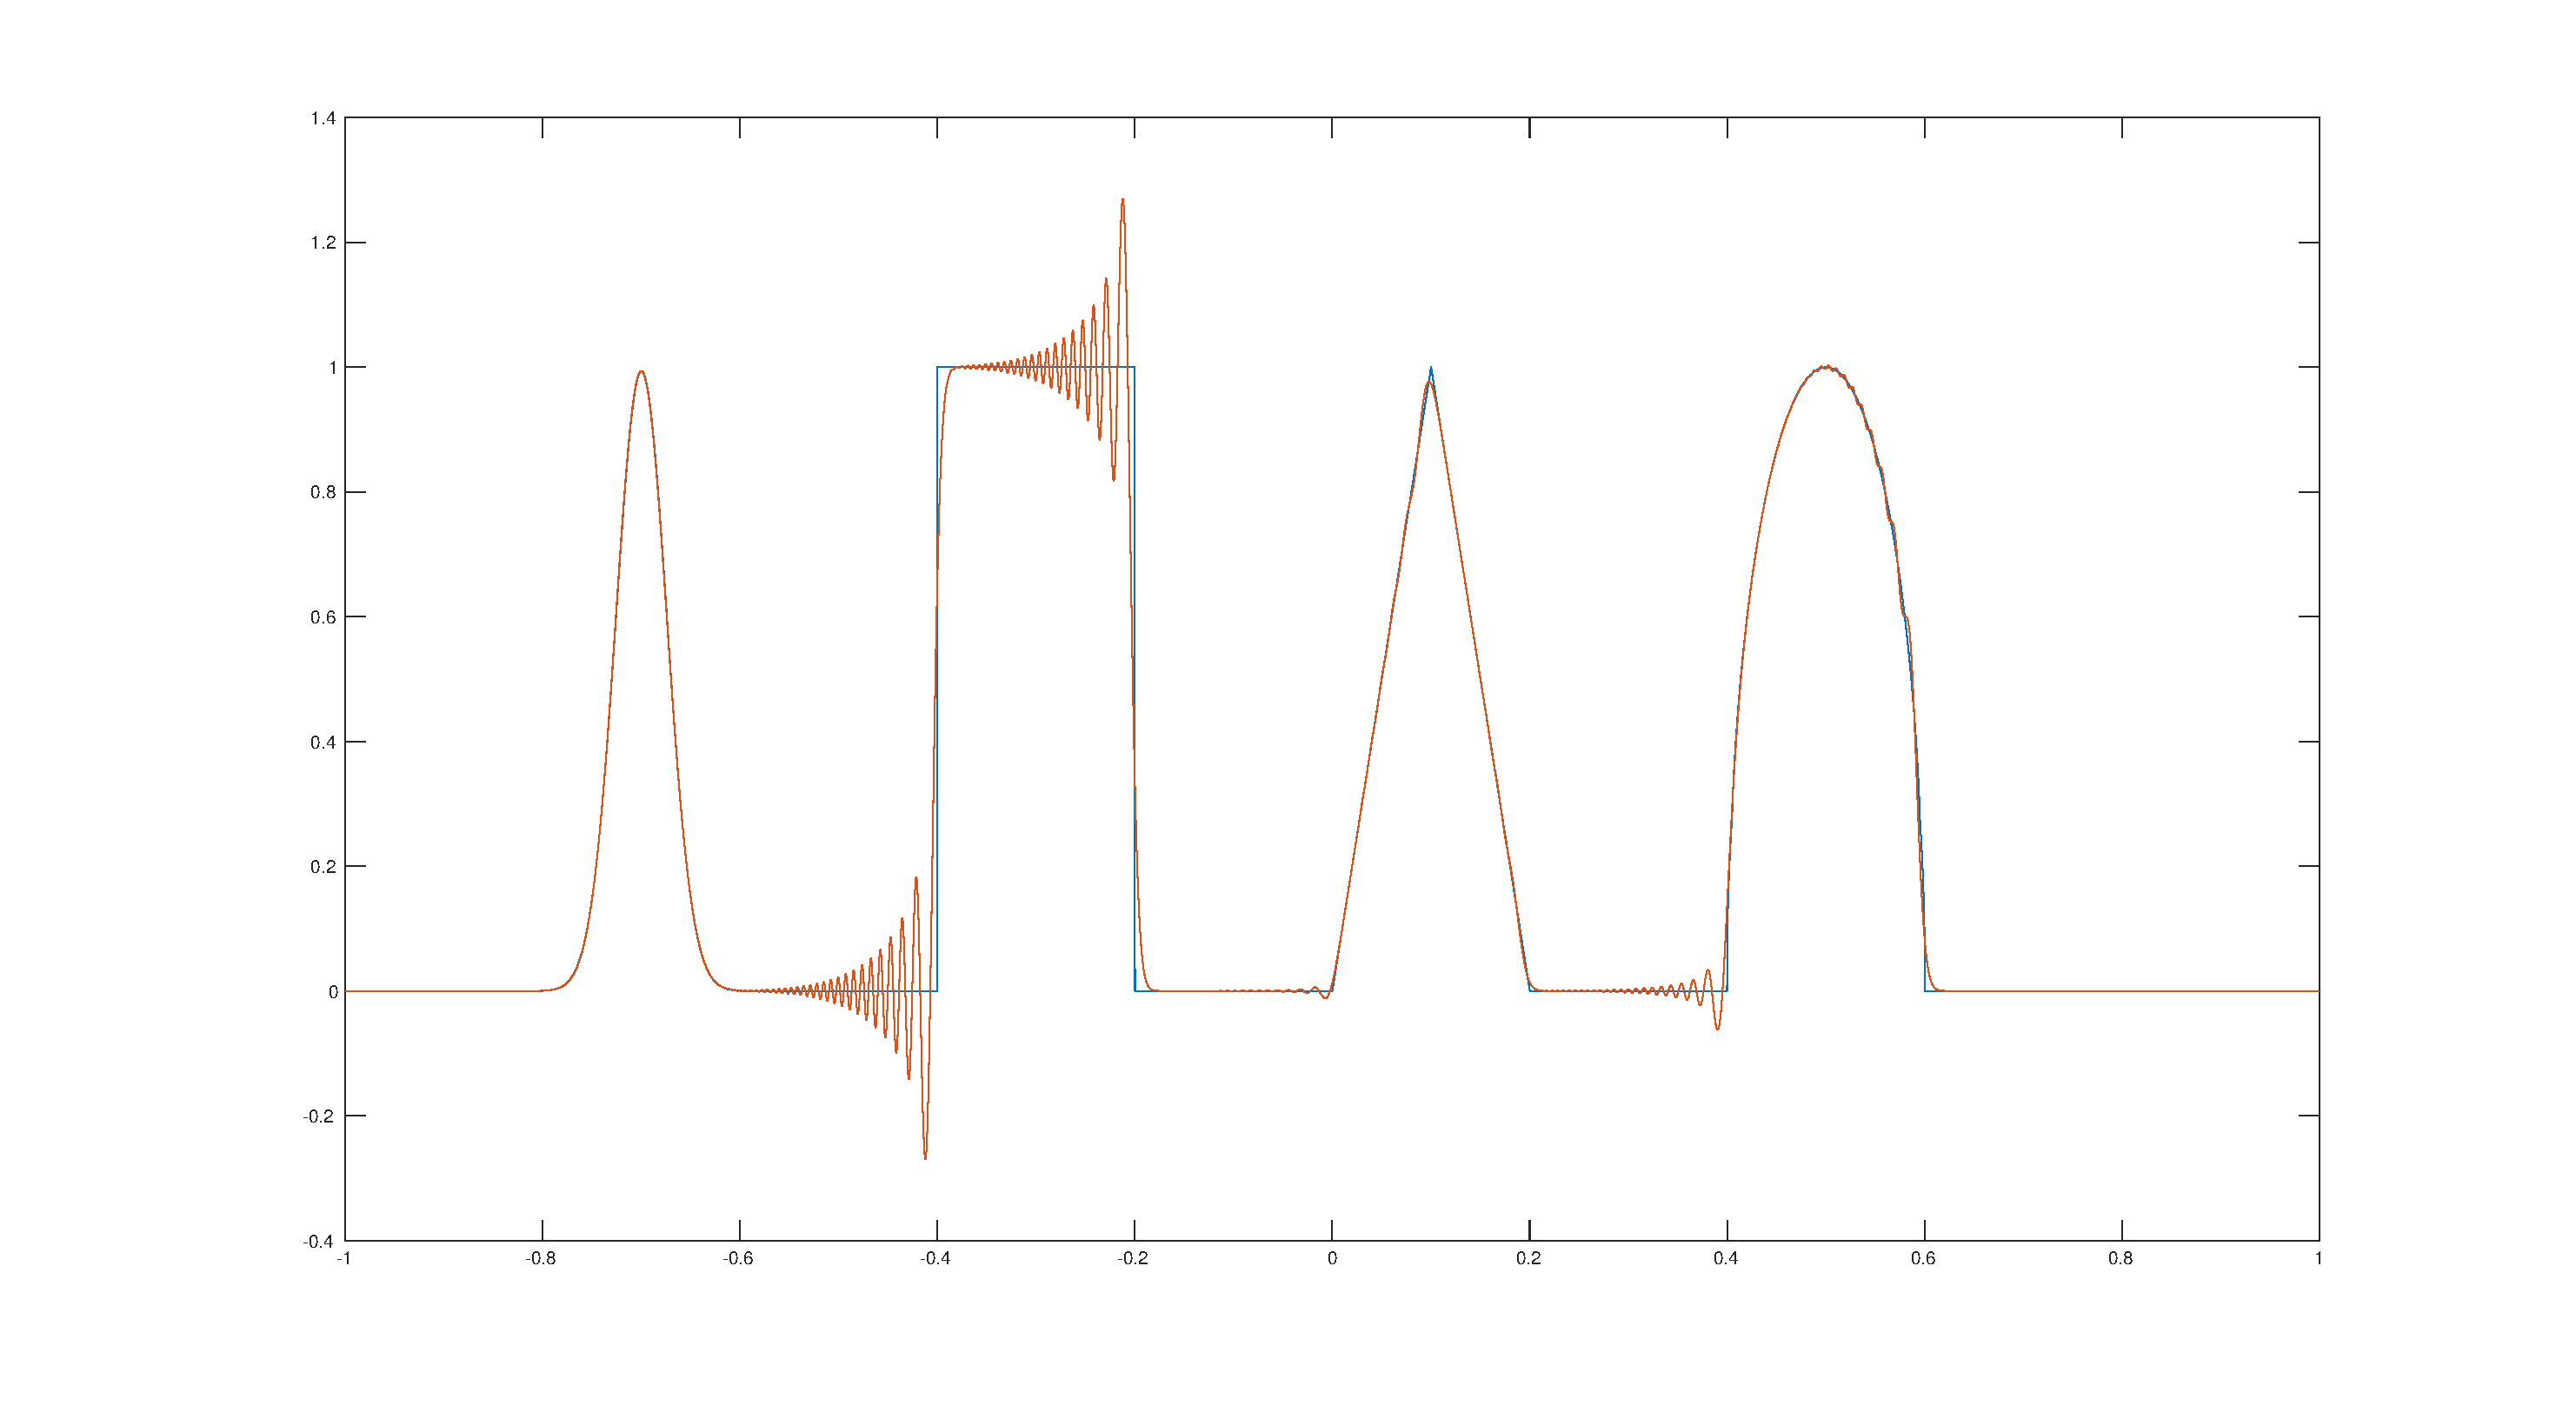
\includegraphics[width=0.45\textwidth,height=0.225\textheight]{./images/advection_LW.eps}
  }
  \subfigure[Force]{
    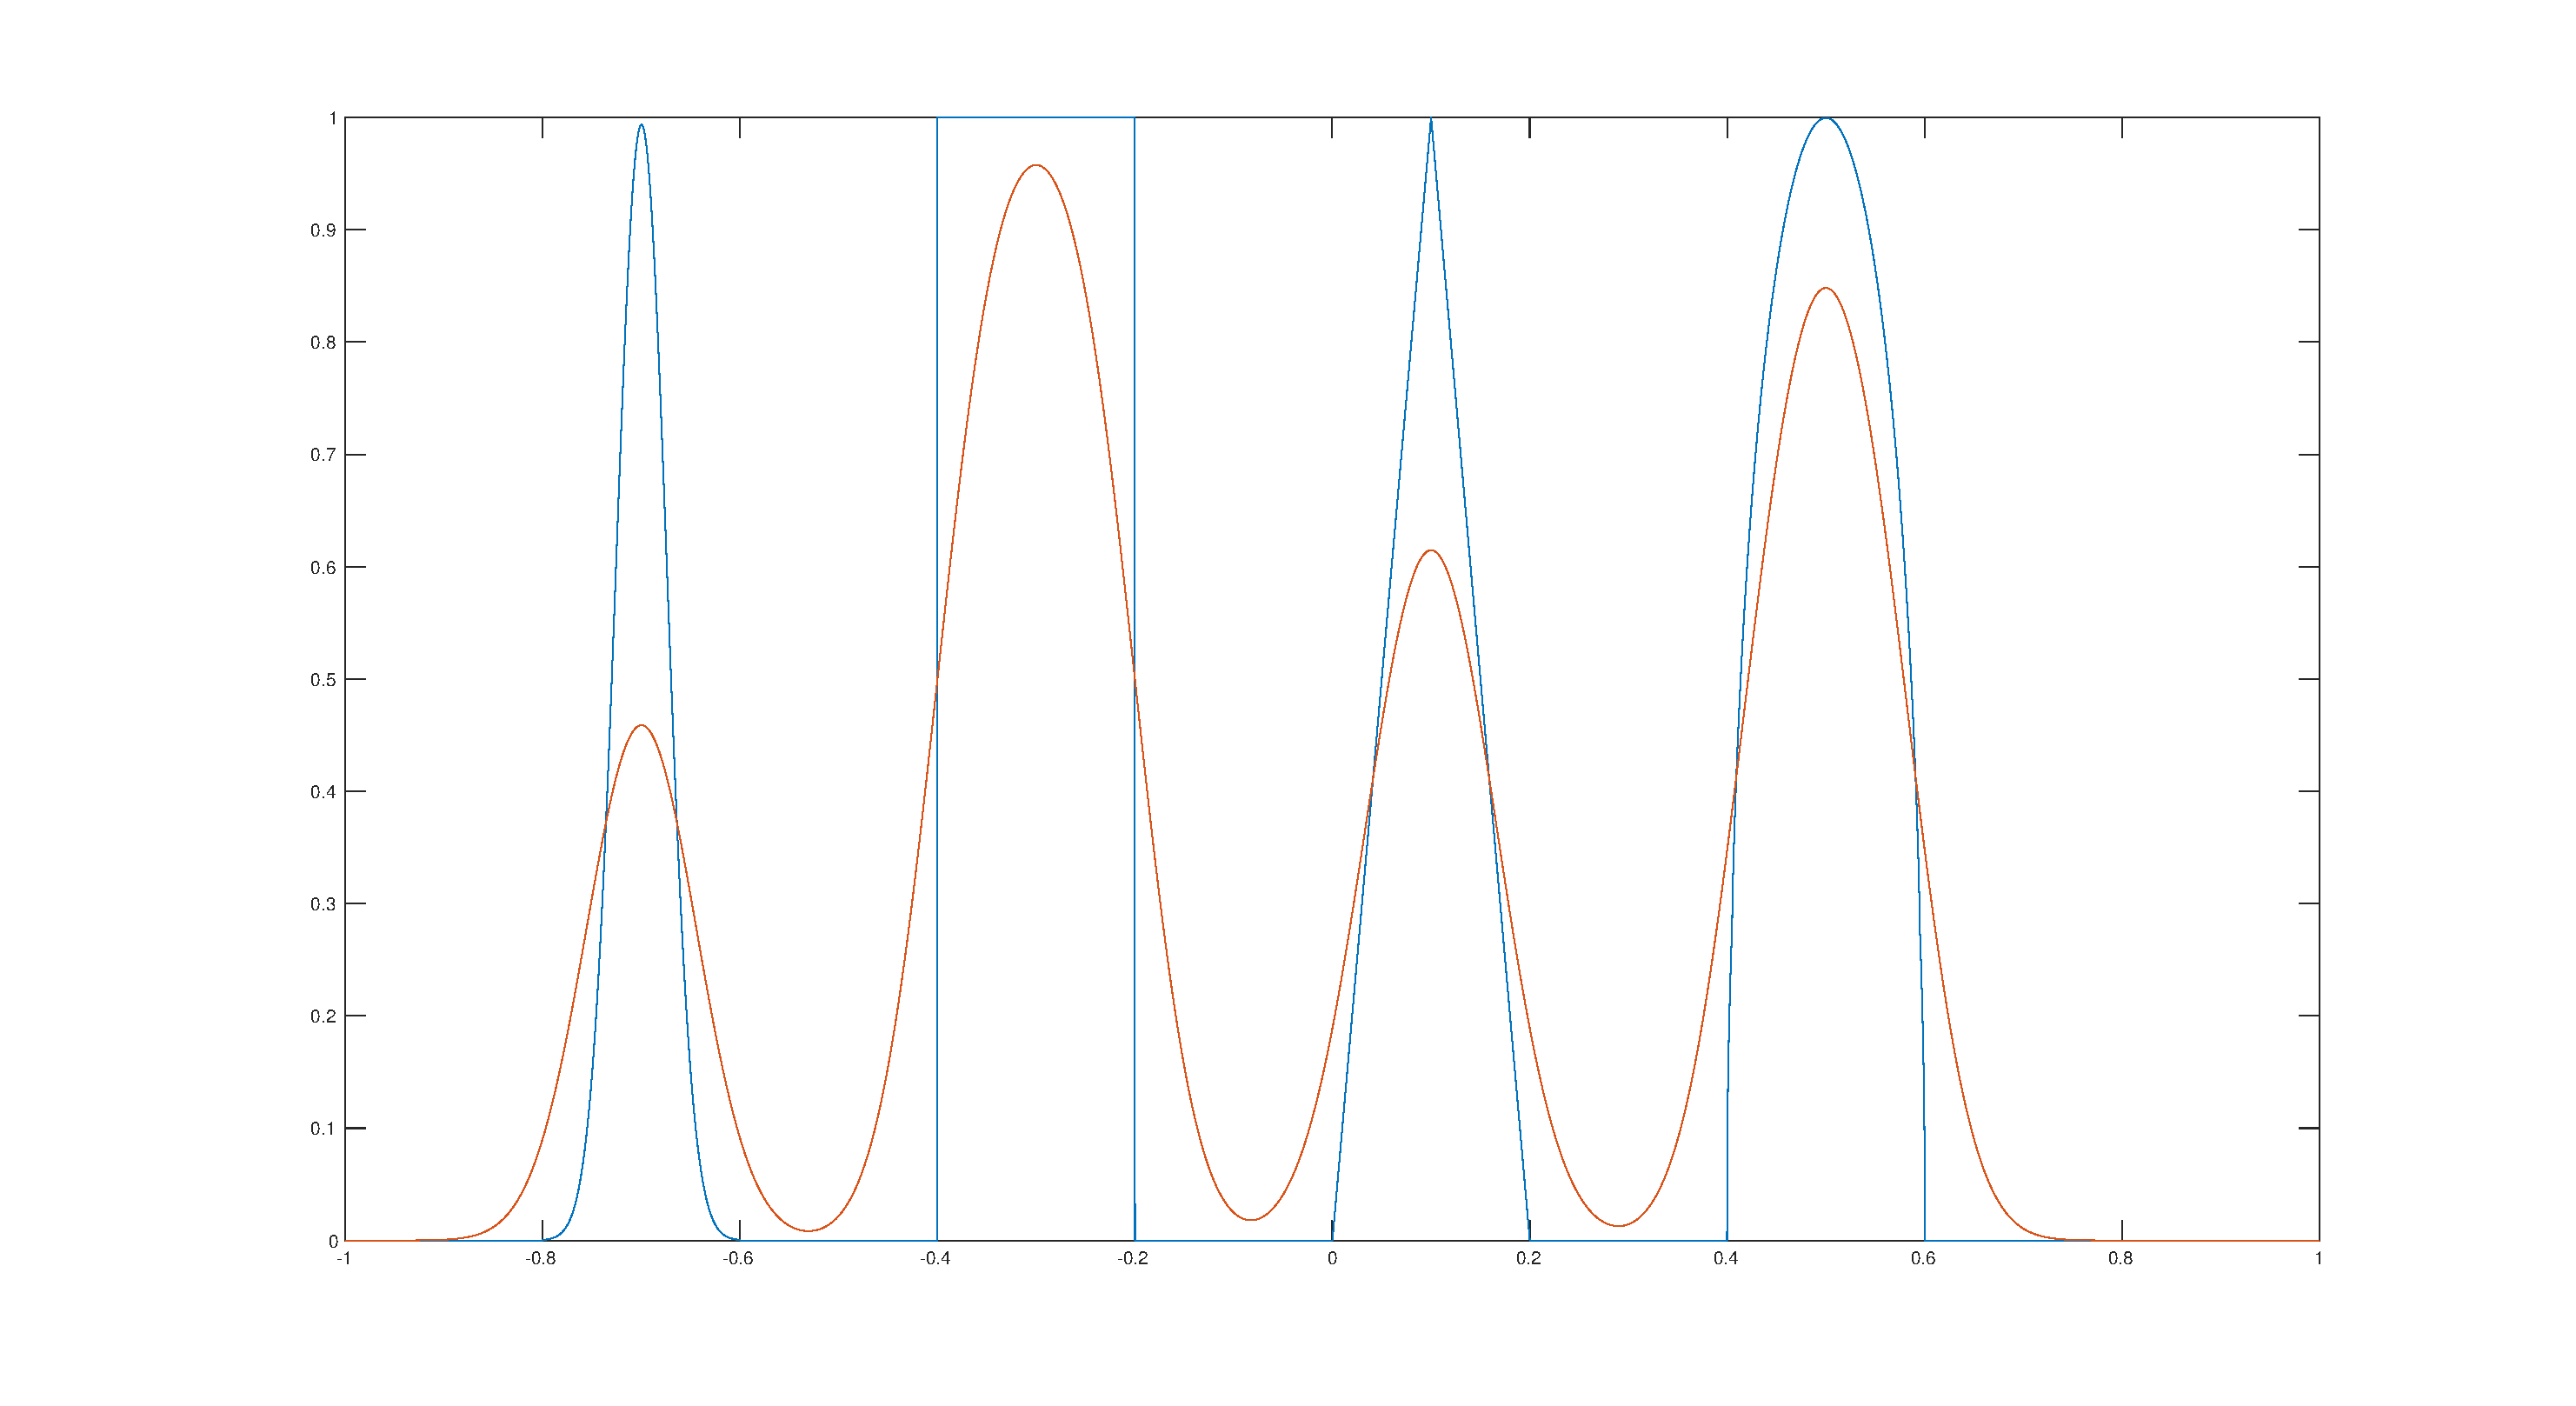
\includegraphics[width=0.45\textwidth,height=0.225\textheight]{./images/advection_Force.eps}
  }
  \subfigure[Godunov]{
    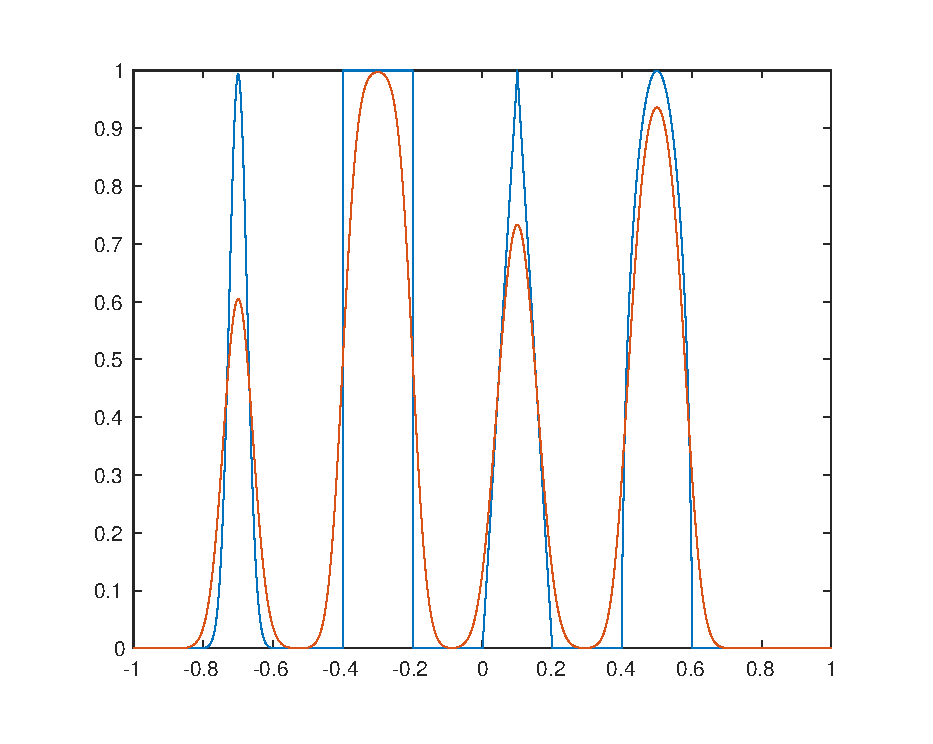
\includegraphics[width=0.45\textwidth,height=0.225\textheight]{./images/advection_Godunov.eps}
  }
\end{figure}
\begin{figure}[H]
  \subfigure[No Reconstruction]{
    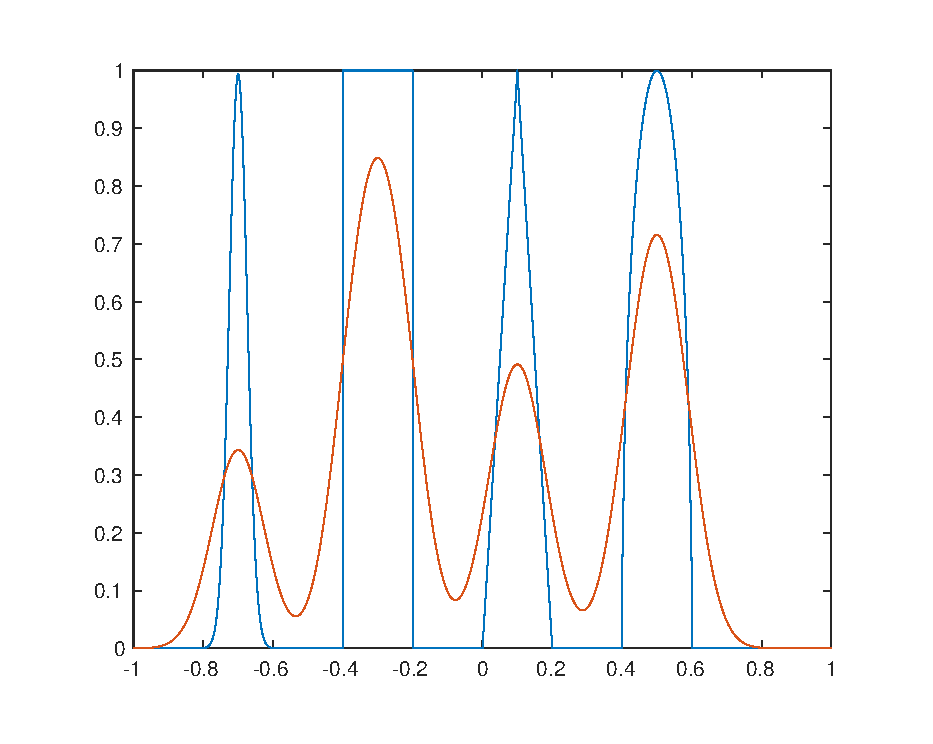
\includegraphics[width=0.45\textwidth, height=0.225\textheight]{./images/advection_LF.eps}
  }
  \subfigure[minmod]{
    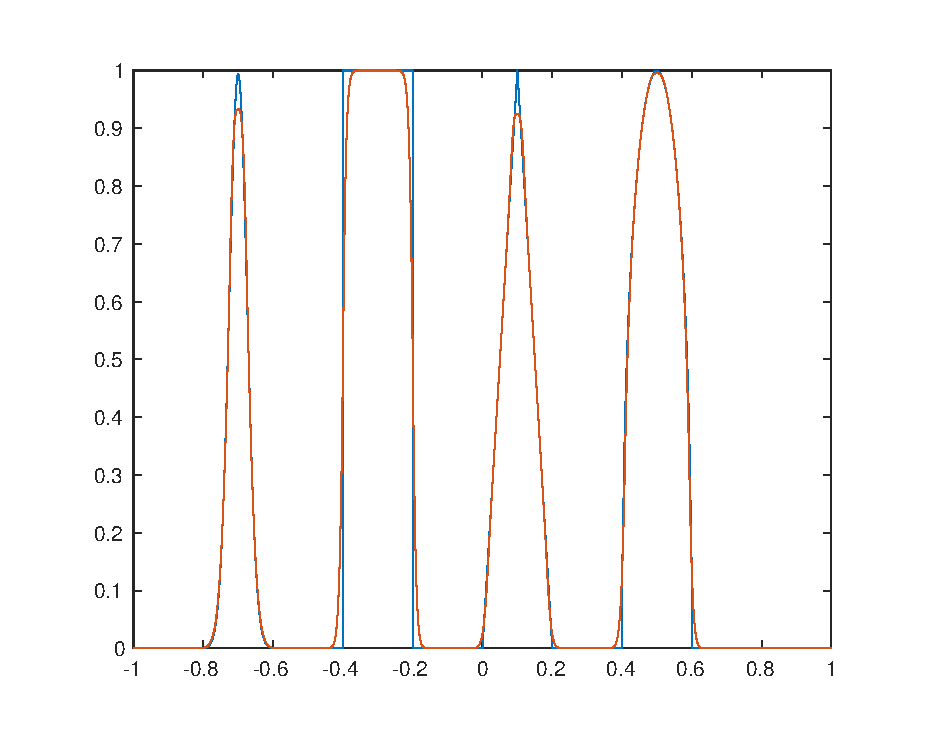
\includegraphics[width=0.45\textwidth,height=0.225\textheight]{./images/advection_LF_minmod_RK.eps}
  }
  \subfigure[superbee]{
    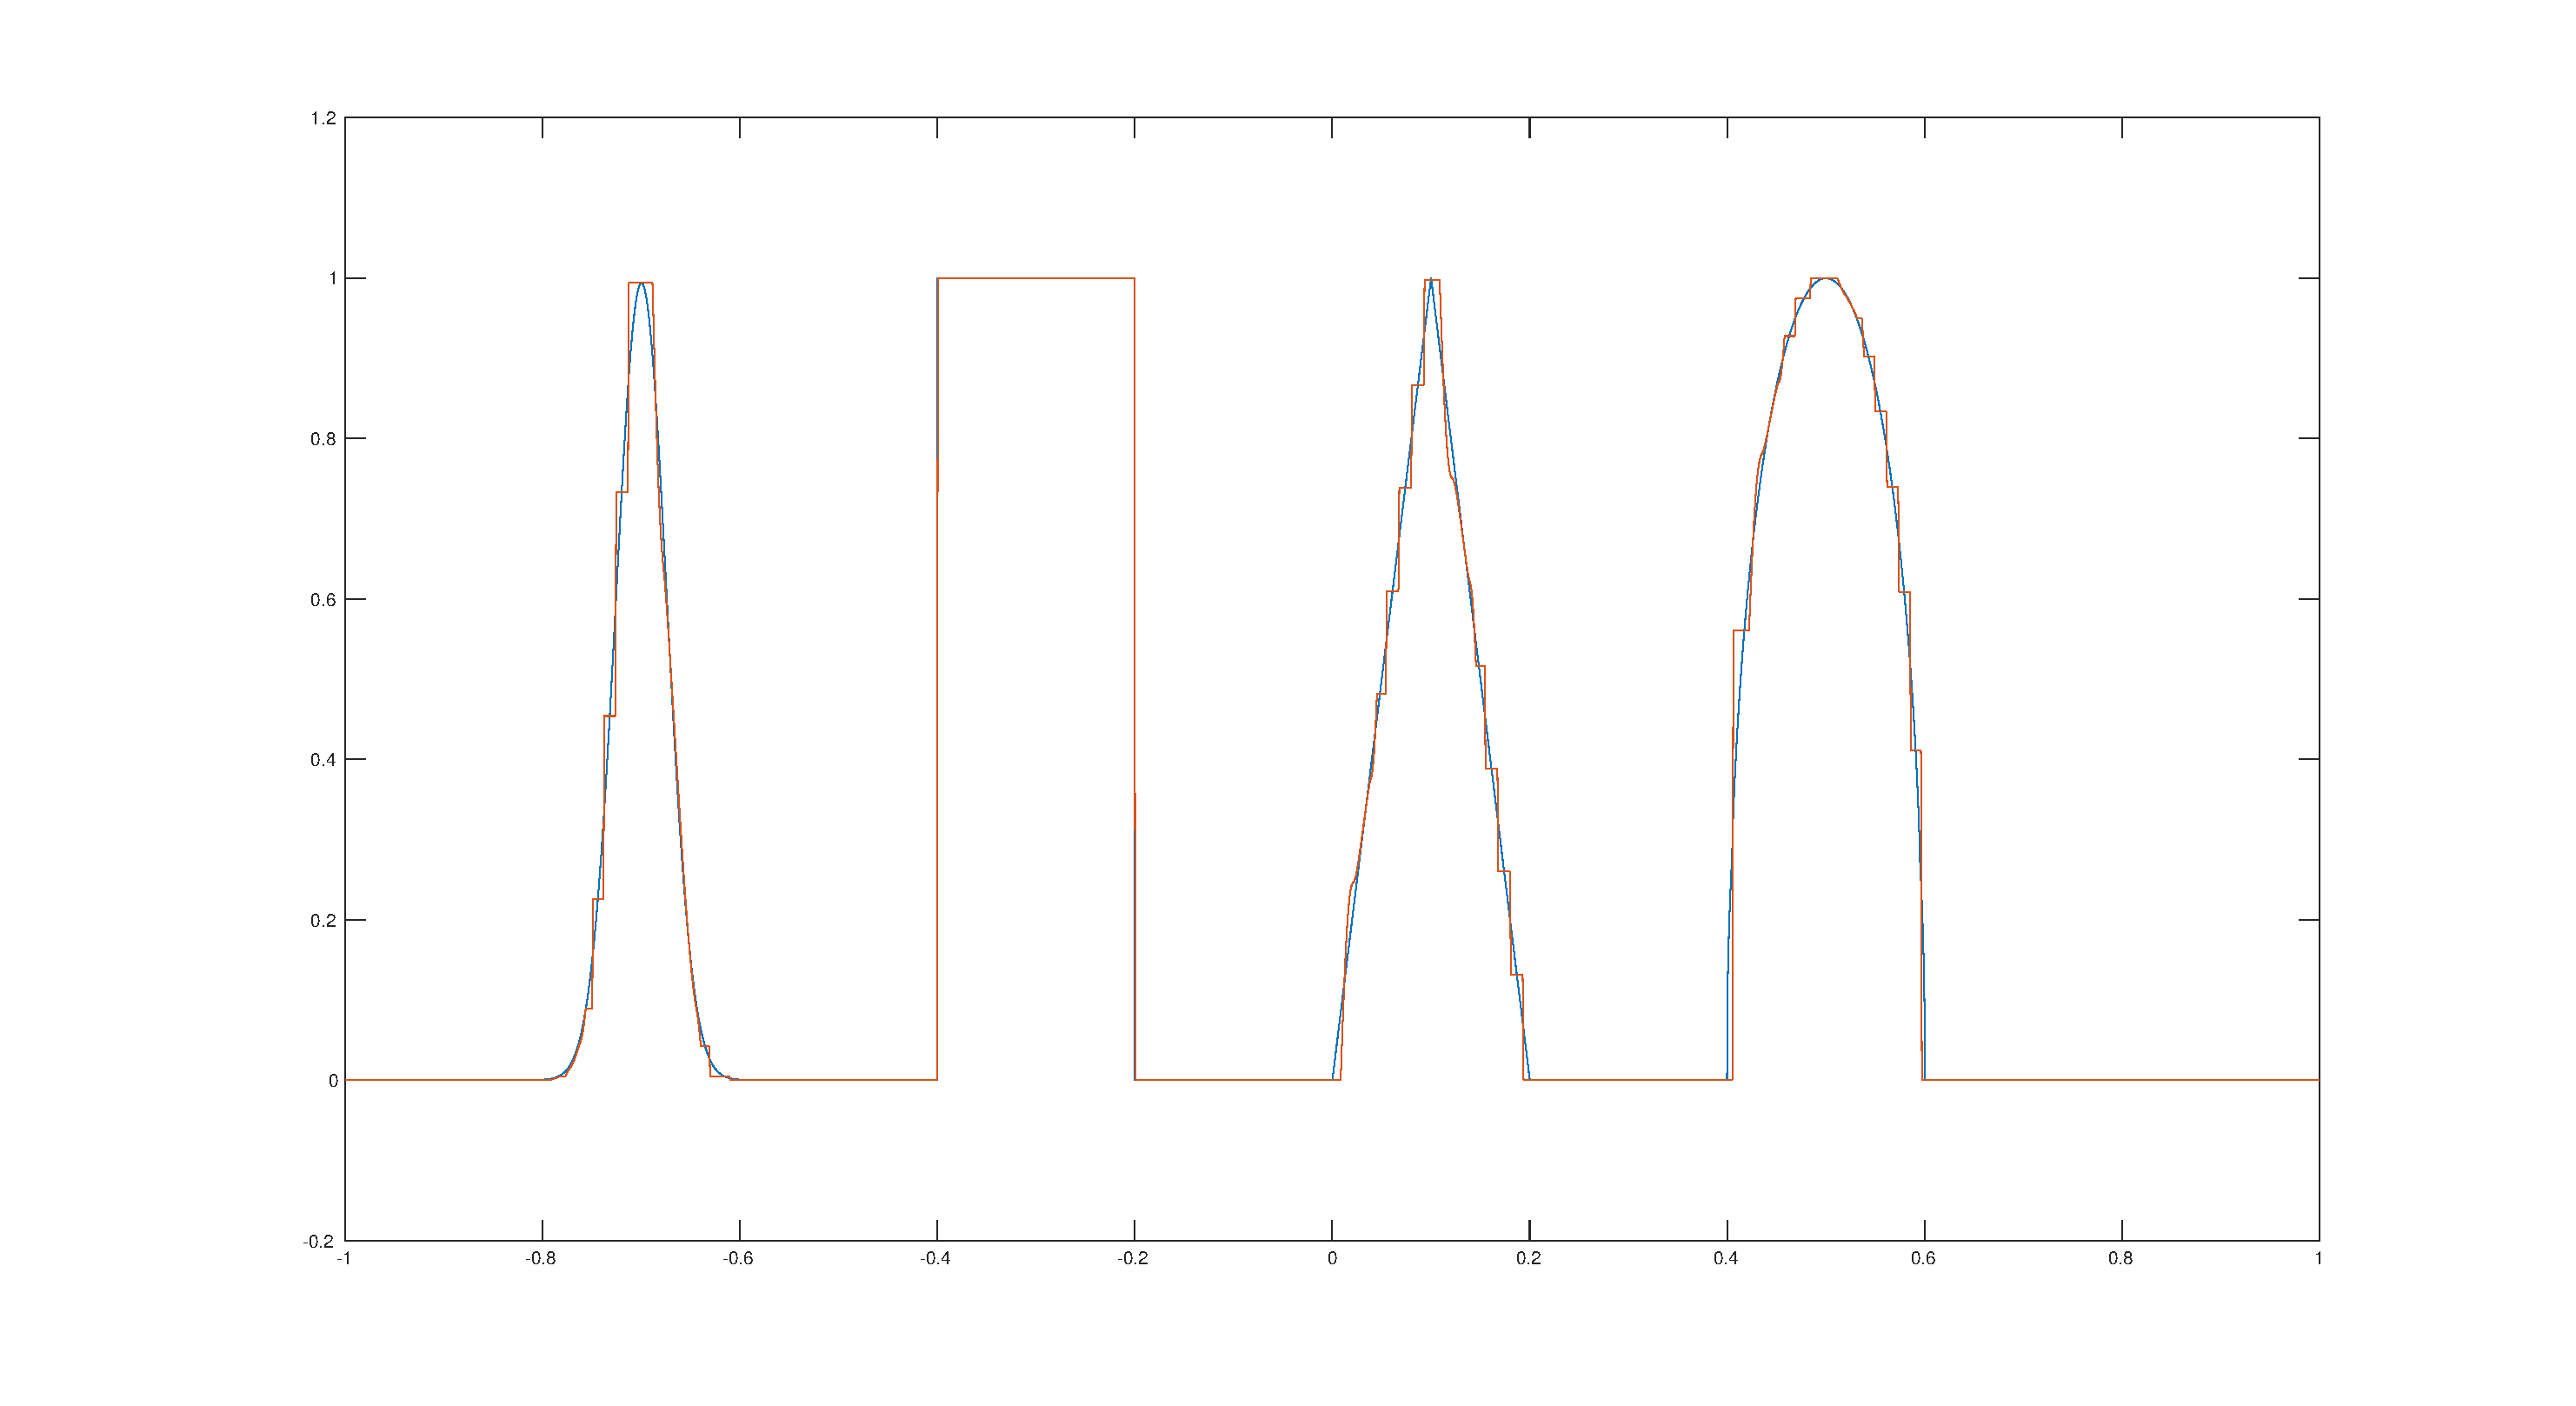
\includegraphics[width=0.45\textwidth, height=0.225\textheight]{./images/advection_LF_superbee_RK.eps}
  }
  \subfigure[MC]{
    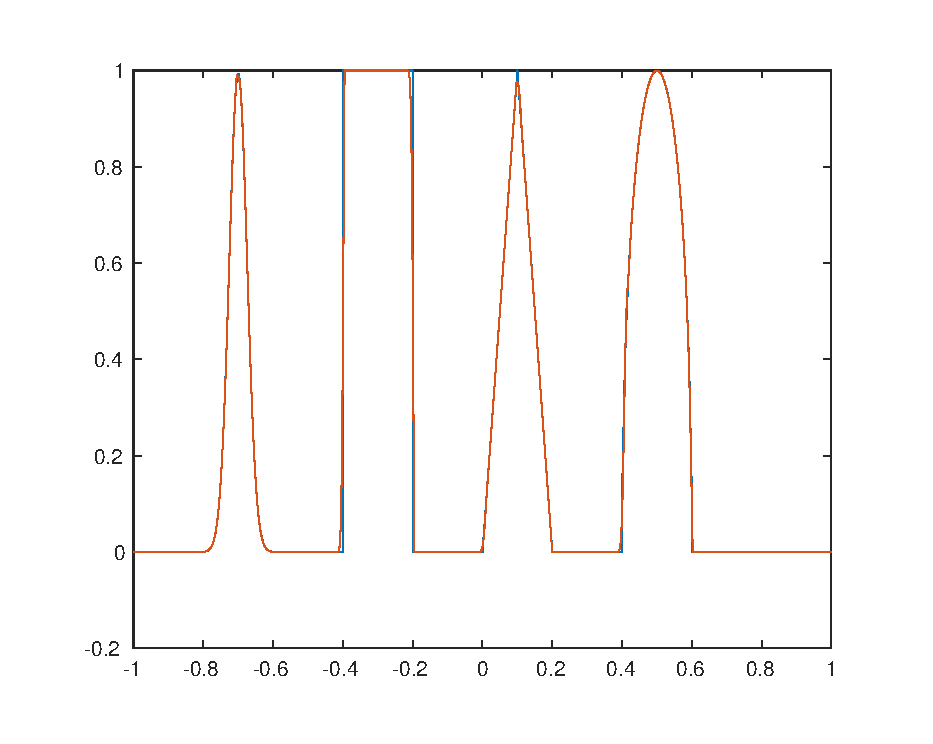
\includegraphics[width=0.45\textwidth,height=0.225\textheight]{./images/advection_LF_MC_RK.eps}
  }

\end{figure}





\subsection{二维问题}



\section{总结}



\end{document}
